\documentclass[11pt,a4paper,leqno]{report}
\usepackage{tikz-cd}
\usepackage{tikz}
%\usepackage[german]{babel}
\usepackage{amsmath}
\usepackage{amsthm}
\usepackage{amssymb}
\usepackage{float}
\usepackage{amsfonts}
\usepackage{hyperref}
\usepackage{lmodern}
%\usepackage{makeidx}
%\usepackage{graphicx}
%\graphicspath{{pics/}}
\usepackage{svg}
\usepackage{amsmath}
\usepackage{delarray}
\makeatletter
\renewcommand*\env@matrix[1][*\c@MaxMatrixCols c]{%
	\hskip -\arraycolsep
	\let\@ifnextchar\new@ifnextchar
	\array{#1}}
\makeatother
\newcommand{\eps}{\varepsilon}
\newcommand{\R}{\mathbb{R}}
\newcommand{\C}{\mathbb{C}}


%%%%%%%%%%% REST %%%%%%%%%%%%%%%%%%%%%%%%%%%%%%%%%%%%

\DeclareMathOperator{\dom}{dom}
\DeclareMathOperator{\ran}{ran}
\newcommand{\re}{\mathrm{Re}}
\newcommand{\im}{\mathrm{Im}}

\newcommand{\ul}{\underline}
\newcommand{\I}{\mathrm{i}}
\newcommand{\E}{\mathrm{e}}

%\makeindex
%\setlength{\parindent}{0em} 


\newtheorem{theorem}{Theorem}[chapter]
\newtheorem{proposition}{Satz}[chapter]
\newtheorem{lemma}[theorem]{Hilfssatz}
\newtheorem{definition}[theorem]{Definition}
\newtheorem{corollary}[theorem]{Folgerung}
\newtheorem{remark}[theorem]{Bemerkung}

\renewcommand{\figurename}{Abbildung}
\numberwithin{equation}{chapter}



\usepackage{listings}
\lstset{basicstyle=\ttfamily}
\lstset{literate=%
	{\"o}{{\"O}}1
	{\"a}{{\"A}}1
	{\"u}{{\"U}}1
	{\"u}{{\"u}}1
	{\"a}{{\"a}}1
	{\"o}{{\"o}}1
}
\renewcommand{\chaptername}{Kapitel}
\renewcommand{\contentsname}{Inhaltsverzeichnis}
\renewcommand{\proofname}{Beweis}
\begin{document}


\begin{titlepage}

\vspace*{5cm}
\begin{center}
\rule{\linewidth}{0.5mm} \\[0.4cm]
{ \Huge \bfseries Elektromagnetismus auf planaren Graphen} \\[0.2cm]
\rule{\linewidth}{0.5mm} \\[3.5cm]
\begin{minipage}[t]{0.4\textwidth}
\begin{flushleft} \large
\emph{Author:}\\
Oliver \textsc{Sko\v{c}ek} \\[4cm]
\small

\end{flushleft}

\end{minipage}
\begin{minipage}[t]{0.4\textwidth}

\end{minipage}
 
% Bottom of the page

 
\end{center}
 
\end{titlepage}

%\maketitle


%\renewcommand{\contentsname}{Contents}

\tableofcontents

\markboth{Contents}{Contents}

\vfill


\chapter*{Einf\"uhrung}
Die Absicht dieser Arbeit ist es ausgehend von der Theorie elektrischer Netzwerke eine Theorie elektromagnetischer Ph\"anomene in der Ebene zu entwickeln. Dabei soll kein Kontinuums\"ubergang gemacht werden sondern allein mit planaren Graphen gearbeitet werden. Zu diesem Zwecke werden einige grundlegende Begriffe der Graphentheorie eingef\"uhrt. Darauf aufbauened werden dann im zweiten Kapitel Funktionnenr\"aume auf diesen Graphen definiert und analog zur mehrdimensionalen Analysis wird eine Theorie mit Analogien zum gewohnten Gradienten, der Divergenz und dem Rotor vorgestellt. Abgeschlossen wird diese Theorie durch ein zum de Rham Komplex analoges Theorem. \\Im dritten Kapitel wird dann ein verallgemeinertes Poissonproblem vorgestellt, dass direkt verwendet werden kann um Widerstandsnetzwerke zu l\"osen. Dies zeigt, dass viele Analogien zwischen dem Problem der Widerstandsnetzwerke und dem Poissonproblem der Elektrostatik existieren.\\
Im vierten Kapitel wird dann eine Version der Maxwell-Gleichungen auf planaren Graphen vorgestellt und zwei wichtige Eigenschaften, Energieerhaltung und Ladungserhaltung behandelt.
Im darauffolgenden Kapitel werden die Maxwellgleichungen in Potentialformulierung vorgestellt und ihre Symmetrie die Eichtransformation vorgestellt.
Im Kapitel "kanonische Quantisierung" wird dann der Sprung von einer klassischen Theorie in eine Quantentheorie gemacht und die Schr\"odingergleichung des Photons konstruiert.

\chapter{Planare Graphen}

	Ein Graph besteht aus Ecken $V$ und Kanten $E$. Die Ecken und Kanten stehen in Beziehung zueinander. Man sagt eine Kante \emph{verbindet} zwei Ecken. Wir wollen nur solche Graphen betrachten, deren Kanten jeweils zwei unterschiedliche Ecken verbinden.
\begin{figure}[H]
	\begin{center}
		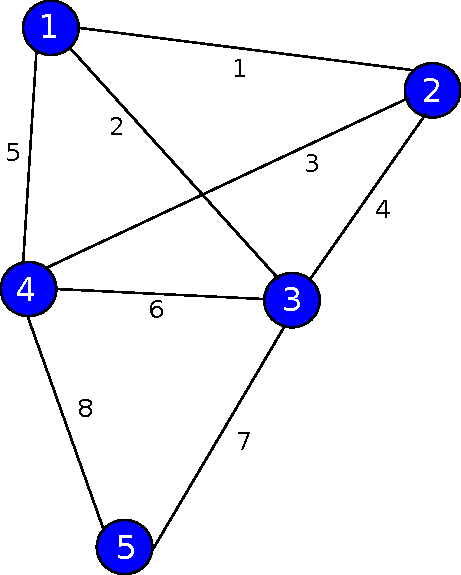
\includegraphics[scale=0.4]{Abbildungen/graph_1.pdf}
		\caption{Beispiel Graph.}
	\end{center}
\end{figure}
\noindent
	Die Beziehung zwischen Ecken und Kanten kann durch eine Matrix dargestellt werden. Der vertikale Index der Matrix steht f\"ur die Kanten und der horizontale Index steht f\"ur die Ecken. Die Matrix ist Eins falls die Kante die Ecke mit einer anderen Ecke verbindet und sonst Null. Diese Matrix nennt man die \textbf{Inzidenzmatrix} des Graphen.\\
	Als Beispiel betrachte die Inzidenzmatrix des Graphen in Abbildung 2.1.
	\begin{center}
		\begin{tabular}{c c c c c}
			1 & 1 & 0 & 0 & 0\\
			1 & 0 & 1 & 0 & 0\\
			0 & 1 & 0 & 1 & 0\\
			0 & 1 & 1 & 0 & 0\\
			1 & 0 & 0 & 1 & 0\\
			0 & 0 & 1 & 1 & 0\\
			0 & 0 & 1 & 0 & 1\\
			0 & 0 & 0 & 1 & 1\\
		\end{tabular} 
	\end{center}
	Im Grunde interessieren wir uns nicht f\"ur die spezielle Realisierung von Ecken und Kanten, sondern f\"ur die Verbindungsstruktur, die genau durch die Inzidenzmatrix festgelegt wird. Dies legt folgende Definition nahe.
\begin{definition}
	Ein \textbf{Graph} ist eine Matrix (Inzidenzmatrix) deren Zeilensumme zwei ist. Zwei Graphen mit Inzidenzmatrizen $X$ und $Y$ sind gleich falls man $X$ aus $Y$ durch Vertauschung von Zeilen und Spalten erhalten kann.
\end{definition}
\begin{remark}
	Alternativ kann ein Graph auch durch eine Adjazenzmatrix definiert werden. Eine solche Matrix ist quadratisch und beide Indizes stehen f\"ur die Ecken des Graphen. Die Adjazenzmatrix ist eins falls die Ecken durch eine Kante verbunden sind und sonst Null. Als Beispiel die Adjazenzmatrix unseres Beispielgraphen.
	\begin{center}
	\begin{tabular}{c c c c c}
		0 & 1 & 1 & 1 & 0\\
		1 & 0 & 1 & 1 & 0\\
		1 & 1 & 0 & 1 & 1\\
		1 & 1 & 1 & 0 & 1\\
		0 & 0 & 1 & 1 & 0\\
	\end{tabular} 
\end{center}
	Der Nachteil der Adjazenzmatrix ist, dass sie keine Mehrfachkanten zwischen zwei Ecken zul\"asst.
\end{remark}
\noindent
Manchmal ist es notwendig \"uber Teile von Graphen zu sprechen. Hierzu dient das Konzept des Teilgraphen. Ein Teilgraph eines Graphen $G$ ist ein Graph, den man durch entfernen von Ecken und Kanten aus $G$ erh\"alt. Bedenke dabei, dass mit jeder Ecke auch alle diese Ecke verbindenten Kanten entfernt werden m\"ussen.
\begin{definition}
	Sei $G$ ein Graph mit Inzidenzmatrix $X$ und $H$ ein Graph mit Inzidenzmatrix $Y$, dann ist $G$ ein \textbf{Teilgraph} von $H$, falls man die Matrix $X$ durch entfernen von Zeilen oder Spalten aus der Matrix $Y$ erhalten kann.
\end{definition}
\noindent
Betrachten wir hierzu einen Teilgraph des Beispielgraphen.
\begin{figure}[H]
	\begin{center}
		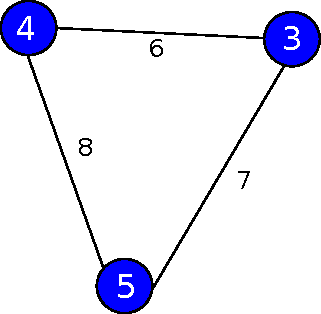
\includegraphics[scale=0.4]{Abbildungen/graph_1_teil.pdf}
		\caption{Teilgraph des Beispielgraphs.}
	\end{center}
\end{figure}
\noindent
Die zugeh\"orige Inzidenzmatrix erhalten wir indem wir die ersten beiden Spalten entfernen und anschlie{\ss}end alle Zeilen, deren Summe ungleich zwei ist. 
\noindent
Das Resultat ergibt dann f\"ur kannten 4, 7 und 8 folgende Inzidenz mit den Ecken 3, 4 und 5.
	\begin{center}
	\begin{tabular}{c c c}
		1 & 1 & 0\\
		1 & 0 & 1\\
		0 & 1 & 1\\
	\end{tabular} 
\end{center}
Eine spezielle Art von Teilgraph erh\"alt man, wenn man eine Teilmenge $U$ der Ecken fixiert und alle Kanten aus dem Graphen entfernt, die eine nicht in der Teilmenge $U$ enthaltene Ecke verbinden. Man nennt so einen Graph den durch die Menge $U$ \textbf{induzierten Teilgraph}. Der Teilgraph in Abbildung 2.2 ist ein solches Beispiel. Es ist der durch $U =\{3, 4, 5\}$ induzierte Teilgraph des Beispielgraphen.
\begin{definition}
	Sei $G$ ein Graph und $n$ eine nat\"urliche Zahl, dann nennt man eine Folge von Ecken $(x_0, x_1,\dots,x_n)$ f\"ur die gilt, dass auf einander folgende Ecken immer durch eine Kante verbunden sind, einen \textbf{Pfad} auf $G$. Falls $x_0 = x_n$ gilt, nennt man dies einenen \textbf{geschlossenen Pfad}. Falls zus\"atzlich bis auf $x_0$ und $x_n$ keine Ecke mehrfach vorkommt, nennt man den Pfad \textbf{einfach geschlossen}.\\
	Man nennt $G$ \textbf{zusammenh\"angend}, falls man von jeder Ecke von $G$ jede andere Ecke \"uber einen Pfad erreichen kann. Sei weiters $k\in\mathbb{N}$, dann sagt man ein Graph ist \textbf{$k$-fach zusammen\-h\"angend}, falls man $k - 1$ beliebige Kanten entfernen k\"onnte und der resultierende Graph immer noch zusammenh\"angend w\"are.
\end{definition}
\noindent
Alle Graphen werden von hier an als zusammenh\"angend angenommen. Allgemein l\"asst sich jeder Graph als Ansammlung von zusammenh\"angenden Teilgraphen darstellen, wodurch diese Annahme im Sinne einer Vereinfachung gerechtfertigt wird.
\begin{definition}
	Ein Graph hat eine \textbf{planare Darstellung} wenn man den Graph auf einem Blatt Papier zeichnen kann, indem man f\"ur jede Ecke einen Punkt zeichnet und f\"ur jede Kante einen Strich zwischen den Eck-Punkten, die sie verbinden soll, ohne das sich dabei zwei Striche kreuzen.
\end{definition}
\noindent
	Der Graph aus Abbildung 2.1 hat eine planare Darstellung. Um dies zu sehen muss man nur die Position von Ecke Nummer 2 ver\"andern.
\begin{figure}[H]
	\begin{center}
		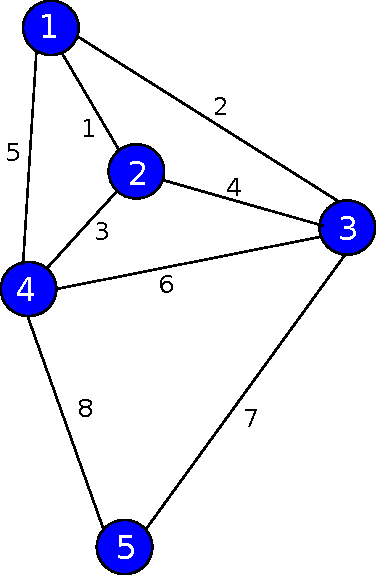
\includegraphics[scale=0.4]{Abbildungen/graph_1_planar.pdf}
		\caption{Beispiel Graph (planar).}
	\end{center}
\end{figure}
\noindent
	Im Allgemeinen gibt es mehrere Wege wie ein bestimmter Graph gezeichnet werden kann. Es gibt sogar f\"ur ein und denselben Graphen oft mehrere planare Darstellungen.
\begin{figure}[H]
	\begin{center}
		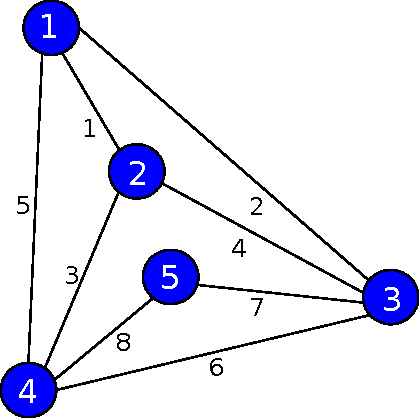
\includegraphics[scale=0.4]{Abbildungen/graph_1_planar2.pdf}
		\caption{Beispiel Graph (planar) alternativ.}
	\end{center}
\end{figure}
\noindent
Es ist also zus\"atzliche Information notwendig um eine planare Darstellung eindeutig festzulegen. Diese zus\"atzliche Information kann \"uber die Fl\"achen aus denen sich die planare Darstellung zusammensetzt gegeben werden.\\
\begin{definition}
	Sei $G$ ein Graph, dann nennt man $G$ einen \textbf{Zyklus} oder \textbf{zyklisch}, falls jede Ecke von $G$ mit genau zwei Kanten verbunden ist.
\end{definition}
\noindent
Betrachten wir eine der planaren Darstellungen des Beispielgraphen. Eine \textbf{Fl\"ache} ist hier ein Zyklus, der keine Ecke einschlie\ss{}t.
\begin{figure}[H]
	\begin{center}
		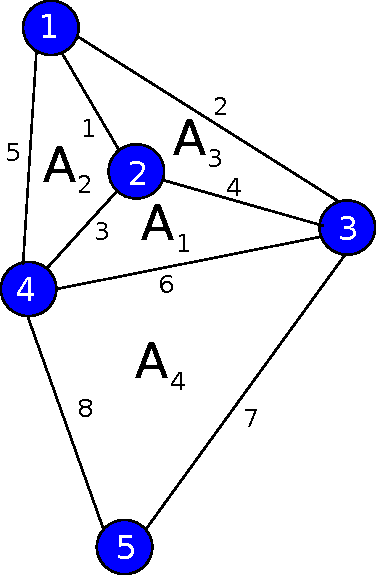
\includegraphics[scale=0.3]{Abbildungen/graph_1_planar_flach.pdf}
		\caption{Beispiel Graph (planar) mit Fl\"achen.}
	\end{center}
\end{figure}
\noindent
\begin{remark}
	Sei $G$ ein Graph und $\{A_1, A_2, \dots, A_n\}$ eine Menge von zyklischen induzierten Teilgraphen, sodass jede Kante von $G$ in maximal zwei der Zyklen vorkommt und jede Ecke von $G$ in mindestens einem der Zyklen vorkommt, dann gibt es eine eindeutige planare Darstellung des Graphen $G$, dessen Fl\"achen genau die $\{A_1, A_2, \dots, A_n\}$ sind.  
\end{remark}
\begin{definition}
	Ein planarer Graph $G=(g, f)$ ist ein Graph $g$ und eine Menge $f$ von Zyklen aus $g$ wie in Bemerkung 1.6. beschrieben. Sei weiters $e$ eine Kante von $g$, dann sagt man $e$ liegt am \textbf{Rand} des Graphen wenn $e$ genau einmal in einer Fl\"ache vorkommt. Der Teilgraph, der genau die am Rand liegenden Kanten enth\"alt nennt man den \textbf{Rand des Graphen}.
\end{definition}
\noindent
Die in Bemerkung 1.6. beschriebene Struktur legt ein mit planaren Graphen eng verkn\"upftes Konzept nahe. Jede Kante des Graphen ist entweder ein Bindeglied zwischen zwei Fl\"achen oder es liegt am Rand des Graphen. Die am Rand liegenden Kanten k\"onnen wiederum als Bindeglied mit der den Graphen umgebenden Fl\"ache, genannt $A_{\infty}$, angesehen werden und somit haben wir das Konzept des dualen Graphen entdeckt.
\begin{definition}
	Es sei $G$ ein planarer Graph, dann kann man einen neuen Graphen, den \textbf{dualen Graph} $G^D$, konstruieren, dessen Kanten mit denen von $G$ \"ubereinstimmen, aber dessen Ecken die Fl\"achen von $G$ zusammen mit der umgebenden Fl\"ache sind, also $V=\{A_1, A_2, \dots, A_n, A_\infty \}$. F\"ur eine gegebene Kante $e$ und Ecke des dualen Graphen $v\in V$ ist die Inzidenzmatrix Eins falls $e$ die Fl\"ache $v$ begrenzt und sonst Null.
\end{definition}
\noindent
Betrachte den dualen Graph des planaren Graphen aus Abbildung 1.5. Beachte die doppelte Kante zwischen Ecke $A_4$ und Ecke $A_\infty$. 
\begin{figure}[H]
	\begin{center}
		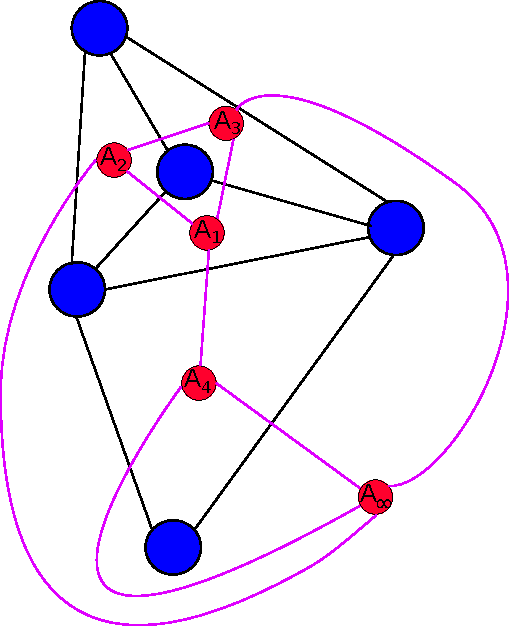
\includegraphics[scale=0.4]{Abbildungen/graph_1_dual.pdf}
		\caption{Dualer Graph des Beispielgraphen.}
	\end{center}
\end{figure}
\noindent
Die blauen Ecken symbolisieren die Ecken des Ausgangsgraphen, während die roten Ecken die Ecken des dualen Graphen darstellen. Die Platzierung von $A_\infty$ ist beliebig gew\"ahlt. Offensichtlich bestimmt diese Wahl, welcher der Ecken des Ausgangsgraphen die umgebende Fl\"ache des dualen Graphen darstellt.
\begin{remark}
	Der duale Graph $G^D$ ist immer auch fast ein planarer Graph, denn jede Ecke von $G$ kann mit einem Zyklus in $G^D$ identifiziert werden, somit bleibt aber offen welche dieser Zyklen, die umgebende Fl\"ache ist. Dies ist insbesondere von Bedeutung wenn man den dualen Graphen des dualen Graphen, den so genannten \textbf{bidualen Graphen} bildet. Um eine eindeutige Zuordnung zu erzwingen muss immer einer der Ecken ausgezeichnet werden oder man verzichtet auf die planare Darstellung und arbeitet mit Polyedern. 
\end{remark}
\noindent
Bislang wurden nur "ungerichtete Graphen" behandelt, also solche deren Kanten keine ausgzeichnete Beziehung mit der einen oder der anderen durch sie verbundenen Ecke haben. Graphen, deren Kanten eine solche Orientierung aufweisen, nennt man "gerichtete Graphen" und eine Adjazenzmatrix ist ein praktisches Weg um solche Strukturen zu beschreiben. Im Gegensatz zur Adjazenzmatrix eines ungerichteten Graphen wird im gerichteten Fall, einfach die Forderung nach Symmetrie der Matrix weggelassen.
\begin{definition}
	Jeder planare Graph kann mit einer \textbf{Orientierung} \\ausgestattet werden, dies ist eine Funktion, die jeder Kante eine der Ecken zuordnet, die durch sie verbunden wird. Man stelle sich vor jede Kante ist ein Pfeil und die Orientierung gibt an auf welche Ecke sie zeigt. Man unterscheidet entsprechend eine \textbf{Spitzefunktion} $x\mapsto p(x)$, welche die Ecke zuordnet, die an der Pfeilspitze liegt und die \textbf{Schaftfunktion} $x\mapsto q(x)$, welche die andere Ecke zuordnet.
\end{definition}
\begin{figure}[H]
	\begin{center}
		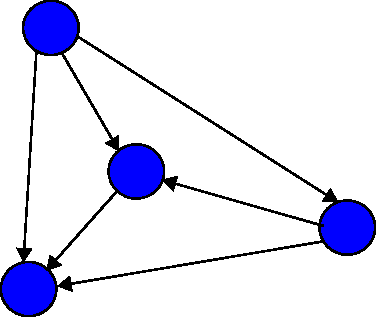
\includegraphics[scale=0.4]{Abbildungen/graph_1_orient.pdf}
		\caption{Graph mit Orientierung.}
	\end{center}
\end{figure}
\noindent
 Zu einem gegebenen Graph gibt es $2^{|E|}$ M\"oglichkeiten, wobei $E$ die Kanten\-menge ist, einen gegebenen Graph mit einer Orientierung auszustatten und ihn hierdurch zu einem gerichteten Graphen zu erheben.
 \begin{remark}
 	Jede Orientierung auf einem planaren Graph $G$, bestimmt eindeutig eine zu ihr \textbf{duale Orientierung} auf dem dualen Graph. Sei hierzu $A$ eine Fl\"ache des planaren Graphen $G$, also ein induzierter Teilgraph, der ein Zyklus ist, und $e$ eine Kante des Graphen, die auch in $A$ liegt, dann setzen wir die Spitzenfunktion $p_D$ der dualen Orientierung $p_D(e) = A$, falls $e$ im planaren Graph $G$ im Uhrzeigersinn bez\"uglich zu $A$ orientiert ist.
 \end{remark}
\begin{figure}[H]
	\begin{center}
		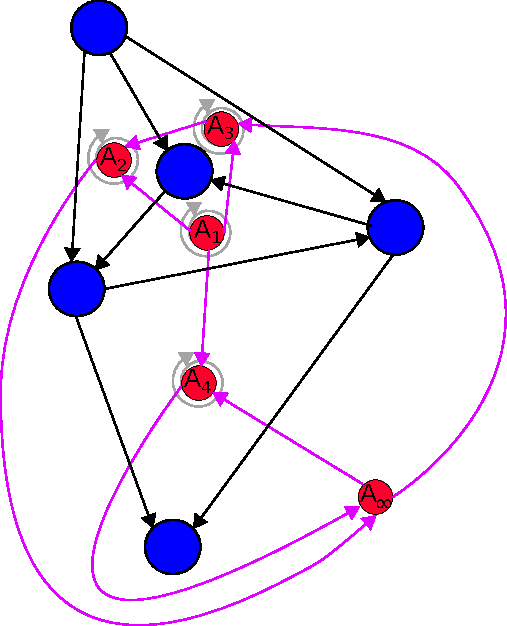
\includegraphics[scale=0.4]{Abbildungen/graph_1_dual_orient.pdf}
		\caption{Orientierung und duale Orientierung.}
	\end{center}
\end{figure}
\noindent

\chapter{Funktionenr\"aume und Operatoren}
Im letzten Kapitel wurden Graphen mit zus\"atzlicher Struktur beschrieben, nämlich planare Graphen und das Konzept des dualen Graphen. In diesem Kapitel sollen die drei Arten von Funktionen auf planaren Graphen und Operatoren, die diese Funktionen aufeinander abbilden vorgestellt werden.
\begin{definition}
	Sei $G$ ein planarer Graph und $G^D$ sein dualer Graph, des weiteren sei $V$ die Menge der Ecken, $E$ die Menge der Kanten und $A$ die Menge der Fl\"achen (inklusive umgebende Fl\"ache), dann unterscheiden wir drei verschiedene (endlichdimensionale) Funktionenr\"aume auf dieser Struktur, den Raum der Kantenfunktionen $\mathfrak{K}=\{f|f: E\rightarrow\mathbb{R}\}$, den Raum der Eckfunktionen $\mathfrak{E}=\{f|f: V\rightarrow\mathbb{R}\}$ und den Raum der Fl\"achenfunktionen $\mathfrak{F}=\{f|f: A\rightarrow\mathbb{R}\}$.
\end{definition}
\noindent
Es gibt eine nat\"urliche Beziehung zwischen diesen drei R\"aumen. 
\begin{definition}
	Sei $G$ ein Graph, $f\in\mathfrak{E}(G)$ eine Eckfunktion auf $G$, seien weiters $p$ und $q$ die Spitzefunktion und Schaftfunktion einer Orientierung auf $G$, dann nennt man $grad(f)\in\mathfrak{K}(G)$ definiert durch 
	$$grad(f)(e) = f(p(e)) - f(q(e))$$ 
	f\"ur eine beliebige Kante $e$ den Gradienten von $f$.
\end{definition}
\begin{definition}
	Sei $G$ ein Graph, $f\in\mathfrak{K}(G)$ eine Kantenfunktion auf $G$, seien weiters $p$ und $q$ die Spitzefunktion und Schaftfunktion einer Orientierung auf $G$, dann nennt man $div(f)\in\mathfrak{E}(G)$, definiert durch: 
	$$div(f)(x) = \sum_{\acute{e}\in E, q(\acute{e})=x}f(\acute{e}) -\sum_{e\in E, p(e)=x}f(e)$$
	f\"ur eine beliebige Ecke $x$ die Divergenz von $f$.
\end{definition}
\noindent
	Der Gradient hebt eine Eckfunktion auf die Kanten, und die Divergenz eine Kantenfunktion auf die Ecken. Der Graph $G$ und der duale Graph $G_D$ haben dieselben  Kantenfunktionen, daher bildet dieser Raum eine Verbindung zwischen Gradient und Divergenz des Graphen und des dualen Graphen. Der Gradient und die Divergenz des dualen Graphen werden durch $grad_D$ respektive $div_D$ symbolisiert. Falls eine Kantenfunktion als Fluss interpretiert wird, entspricht die Divergenz der Kantenfunktion dem Nettofluss von den Ecken weg.
\begin{proposition}
		Sei $G$ ein planarer Graph mit Orientierung, dann sind der Gradient und die Divergenz lineare Operatoren und es gilt:
		$$div = -grad^T$$
		wobei sich die Adjunktion auf das Standardskalarprodukt bezieht.
\end{proposition}
\begin{proof}
Sei $u\in\mathfrak{E}(G)$ und $v\in \mathfrak{K}$, dann schreiben wir das Skalarprodukt:
$$\langle v, \text{grad}(u)\rangle_\mathfrak{K} = \sum_{x\in E} v(x) * (u(p(x) - u(q(x)))) = $$
$$\sum_{x\in E} v(x) * u(p(x)) - \sum_{x\in V} v(x) * u(q(x))=$$
$$\sum_{e\in V} u(e) * \sum_{j\in E, p(j)=e}v(j) - \sum_{e\in V} u(e) * \sum_{j\in E, q(j)=e}v(j) =$$
$$-\langle \text{div}(v), u\rangle_\mathfrak{E}$$
\end{proof}
\begin{definition}
	Sei $G$ ein planarer Graph mit Orientierung und $f\in\mathfrak{K}(G)$, $(x_i)_{i=1}^n$ ein Pfad auf $G$, $(e_i)_{i=1}^{n-1}$ die Folge der Kanten, die f\"ur jedes $1\leq i \leq n-1$ $x_i$ und $x_{i+1}$ verbinden und es sei $\sigma_i$ f\"ur jedes $1\leq i \leq n-1$ gleich $-1$ falls $p(e_i)=x_i$ ist und sonst $+1$, dann nennt man die Summe
	$$ \sum_{i=1}^{n-1} \sigma_i f(e_i)$$
	die \textbf{Pfadsumme.}
\end{definition}
\begin{proposition}
	Sei $G$ ein planarer Graph mit Orientierung, $f\in\mathfrak{K}(G)$ sodass $\text{div}_D(f)=0$, dann gilt dass f\"ur jeden geschlossenen Pfad in $G$ die Pfadsumme gleich Null ist.
\end{proposition}
\begin{proof}
Zu allererst reicht es einfach geschlossene Pfade zu betrachten. Diese Einschränkung ist zul\"assig weil sich f\"ur alle anderen geschlossenen Pfade die Pfadsumme sich als Summe solcher einfach geschlossenen Pfade schreiben l\"asst.\\
\\
Jeder einfach geschlossene Pfad zerteilt den Graph in zwei Teilgraphen, sodass die Vereinigung der Teilgraphen ganz $G$ ist und der Durchschnitt nur den geschlossenen Pfad enth\"alt. Jener Teilgraph, der keinen Teil des Randes von $G$ enth\"alt ist der innere Graph.\\
\\
Sei $f\in\mathfrak{K}(G)$, dann gilt f\"ur jeden Zyklus in $G$, dass falls er als Pfad gegen den Uhrzeigersinn orientiert geschrieben wird, die Pfadsumme gleich dem Wert von $\text{div}_D$ ist.\\
\\
Sein nun $(x_i)_{i=1}$ ein einfach geschlossener Pfad, dann k\"onnen wird die Pfad- summe als Summe \"uber alle Zyklen des zugeh\"origen inneren Graphen schreiben, da die Pfade \"uber die Zyklen immer als gegen den Uhrzeigersinn orientiert angenommen werden, heben sich alle Kantenwerte auf, die nicht zum Pfad $(x_i)_{i=1}$ geh\"oren.
Da $\text{div}_D(f)=0$ ist, ist somit auch die Pfadsumme gleich Null.
\end{proof}
\noindent
	Es besteht eine Analogie der hier definierten Operatoren zu den Differential\-operatoren der Vektoranalysis. Interessanterweise entspricht die duale Divergenz der Rotation. Die Analogie untermauernd kann man folgendes Theorem formulieren.
\begin{theorem}[Der de Rham Komplex]
	Die Operatoren $grad$, $div$, $grad_D$ und $div_D$ erf\"ullen folgende exakte Sequenzen, daher das Bild der Abbildungen entspricht dem Kern der nachfolgenden Abbildung. Beachte, dass $\mathbb{R}$ in den Formeln f\"ur die dem entsprechenden Raum zugeh\"origen konstanten Funktionen steht.
\begin{equation}
	\mathbb{R}\longrightarrow\mathfrak{E}(G) \overset{grad}{\longrightarrow}\mathfrak{K}(G) \overset{div_D}{\longrightarrow}\mathfrak{F}(G)/\mathbb{R}\longrightarrow 0
\end{equation}
\begin{equation}
	\mathbb{R}\longrightarrow\mathfrak{F}(G) \overset{grad_D}{\longrightarrow}\mathfrak{K}(G) \overset{div}{\longrightarrow}\mathfrak{E}(G)/\mathbb{R}\longrightarrow 0
\end{equation}
\end{theorem}
\begin{proof}[Beweis de Rham Komplex]
	Es gen\"ugt Gleichung 2.1 in Theorem 2.4 zu beweisen, da 2.2 durch Anwendung von 2.1 auf den dualen Graphen folgt.\\
	\\
	\textbf{Erste zu beweisende Aussage:} Der Kern von $\text{grad}$ ist genau der Raum der konstanten Eckfunktionen.\\
	\\
	Da $G$ zusammenh\"angend ist und da $\text{grad}$ an einer Kante nur Null sein kann wenn beide Ecken, welche die Kante verbindet, den selben Wert haben, ist $\text{grad}(f)$ genau dann Null wenn $f$ konstant ist.\\
	\\
	\textbf{Zweite zu beweisende Aussage:} Das Bild von $\text{grad}$ ist genau der Kern von $\text{div}_D$.\\
	\\
	Sei $a$ ein Zyklus von $G$, und $(x_i)_{i=1}^k$ ein Pfad der die Ecken des Zyklus gegen den Uhrzeigersinn durchl\"auft und $f\in\mathfrak{E}$, dann gilt:
	$$div_D(\text{grad}(f)) = \sum_{i=1}^{k-1} \sigma(i) * \overbrace{\sigma(i) * (f(x_{(i+1) \text{ mod } k})-f(x_{i  \text{ mod } k}))}^{\text{grad}}$$
	Da ja $k \text{ mod }k=0$ gilt, kommt in der Summe jeder Wert von $f$ genau einmal mit positiven und einmal mit negativen Vorzeichen vor. Daher die Summe ist gleich Null.\\
	\\
	Es fehlt noch zu zeigen, dass jedes Element im Kern von $\text{div}_D$ auch im Bild von $\text{grad}$ ist.\\
	\\
	Sei $f$ eine Kantenfunktion, sodass gilt $\text{div}_D(f)=0$, dann gilt wegen dem Satz 2.2, dass f\"ur beliebige Ecken $a, b\in V$ gilt, dass die Pfadsummen f\"ur alle Pfade, die in $a$ starten und in $b$ enden, gleich sind.\\
	\\
	W\"ahlen wir nun eine beliebige Ecke $x_0$, weil $G$ zusammenh\"angend ist, k\"onnen wir von $x_0$ zu jeder Ecke in $G$ einen Pfad bilden um $F\in\mathfrak(E)(G)$ zu definieren, sodass f\"ur jede Ecke $x$ $F(x)$ gleich der Pfadsumme eines Pfades von $x_0$ nach $x$ hat. Dies ist ja eindeutig. Es gilt nun $\text{grad}(F) = f$.
	\\
	\\
	\textbf{Die letzte zu beweisende Aussage:} Das Bild von $\text{div}_D$ ist genau das orthogonale Komplement der konstanten Fl\"achenfunktionen.\\
	\\
	Wegen des Satzes 2.1 und der ersten Aussage in diesem Beweis folgt die Aussage.
\end{proof}
\noindent
\chapter{Das Poisson Problem}
Ein klassisches Problem der Theorie elektrischer Netzwerke sowie der Elektrostatik ist das (verallgemeinerte) Poissonproblem. Dieses Problem wird hier in einigen seiner Facetten vorgestellt und basierend auf der bisher behandelten Graphentheorie formuliert und gel\"ost.
\paragraph{Das verallgemeinerte Poisson Problem}
Sei $G$ ein Graph, $\partial$ eine Teilmenge der Ecken, $r$ eine positive Kantenfunktion und $f$ und $g$ Eckfunktionen, dann wird eine Eckfunktion $u$ gesucht sodass gilt:

\begin{align}
	-div(r * grad(u))(x) = f(x)\text{  falls } x\notin \partial\\
	u(x) = g(x)\text{  falls } x\in \partial
\end{align}
Die Bedingung 3.2 ist motiviert durch Randwertprobleme aus der Theorie der partiellen Differential\-gleichungen.
\begin{definition}
	Sei $G$ ein planarer Graph mit Orientierung, $r$ eine positive Kantenfunktion, dann nennt man $\Delta_r$, definiert durch 
	$$\Delta_r(u) = -div(r * grad(u))\text{ falls }u\in\mathfrak{E}(G)$$
	den \textbf{$r$-gewichteten Laplace} Operator
\end{definition}
\paragraph{Die Formulierung f\"ur elektrische Netzwerke}Gegeben ein Netzwerk(Graph) bestehend aus Spannungsquellen, Stromquellen und linearen Komponenten (elektrische Widerst\"ande), finde  die elektrische Spannung zwischen beliebigen zwei Punkten im Netzwerk, und f\"ur jeden Leiter im Netzwerk, den durch\-flie\ss{}enden elektrischen Strom.
\begin{figure}[H]
	\begin{center}
		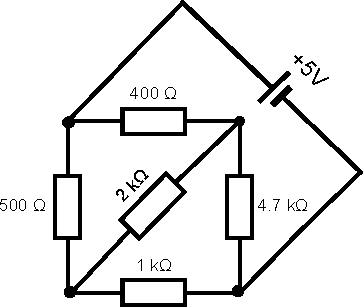
\includegraphics[scale=0.6]{Abbildungen/stromkreis_1.pdf}
		\caption{Beispiel Stromkreis.}
	\end{center}
\end{figure}
\noindent
\paragraph{Die Formulierung in der Elektrostatik} Sei $\Omega$ eine offene Teilmenge des $\mathbb{R}^3$ mit glatten Rand $\partial\Omega$ und $\rho$ die elektrische Ladungsdichte in $\Omega$. Gesucht ist das Potential $\phi:\Omega\rightarrow\mathbb{R}$ sodass:
\begin{align}
\Delta \phi(x) = \rho(x)\text{  falls } x\in \Omega\\
\phi(x) = 0\text{  falls } x\in \partial\Omega
\end{align}
Physikalisch wird $\Omega$ ein Hohlraum in einem guten elektrischen Leiter, wie etwa einem Metall, sein,  da ein Solcher das Potential am Rand des Hohlraumes auf einen konstanten Wert zwingt.\\
\\
Die Elektrostatik lebt im $\mathbb{R}^3$, daher ist die bisher entwickelte Theorie nur in Grenzf\"allen anwendbar. Dieser Spezialfall tritt ein falls $\rho$ und $\Omega$ o.B.d.A entlang der z-Achse konstant sind, daher das Problem effektiv zwei Dimensional wird. F\"ur genau diesen Fall wird eine Theorie der zweidimensionalen Maxwell-Gleichungen im n\"achsten Kapitel entwickelt. 
\begin{proposition}
	Sei $G$ ein  Graph, $r$ eine positive Kantenfunktion und $\Delta_r$ der $r$-gewichtete Laplace Operator, dann gilt:
	\begin{itemize}
		\item Die Form der Matrix $\Delta_r$ is unabh\"angig von der gew\"ahlten Orientierung auf $G$. 
		\item $\Delta_r$ ist symmetrisch.\\
		\item $\Delta_r$ ist positiv semidefinit.\\
		\item Der Kern von $\Delta_r$ ist der Raum der konstanten Eckfunktionen.
	\end{itemize}
\end{proposition}
\begin{proof}
	Seien $p_0$ und $p_1$ Orientierungen auf $G$ und $grad_0$ und $grad_1$ die zugeh\"oringen Gradienten, dann gilt:
	$$grad_0 = D * grad_1$$
	wobei $D$ eine Diagonalmatrix ist, deren Eintr\"age $\pm 1 $ sind. Wegen Satz 2.1 folgt die erste Aussage.\\
	\\
	Die zweite Aussage folgt direkt aus der Definition von $\Delta_r$ und Satz 2.1. Seien hierzu $u$ und $v\in\mathfrak{E}$, dann gilt:
	$$\langle u, \Delta_r(v)\rangle_\mathfrak{E} = \langle \sqrt{r}*\text{grad}(u), \sqrt{r}*\text{grad}(v)\rangle_\mathfrak{K}$$
	Analog zeigt man die dritte Aussage, indem man $u=v$ setzt.
	$$\langle \sqrt{r}*\text{grad}(u), \sqrt{r}*\text{grad}(u)\rangle_\mathfrak{K}\geq 0$$
	Die letzte Aussage: $u\in\text{kern}(\Delta_r)$ gilt genau dann wenn f\"ur jedes $v\in\mathfrak{E}$
	$$\langle v, \Delta_r(u)\rangle_\mathfrak{E}=0$$
	also genau dann wenn
	$$\langle \sqrt{r}*\text{grad}(u), \sqrt{r}*\text{grad}(v)\rangle_\mathfrak{K}=0$$
	Da $r>0$ gilt, ist dies equivalent zu der Aussage $u\in\text{kern}(\text{grad})$. Der Gradient ist genau dann Null wenn $u$ konstant ist, da unser Graph zusammenh\"angend ist.
\end{proof}
\noindent
In der kontinuierlichen Theorie des Poissonproblems sind Sobolevr\"aume und die Poincare Ungleichung von zentraler Bedeutung. Ein Analogon gibt es nat\"urlich auch in der diskreten oder graphischen Theorie.
\begin{proposition}[Poincare Ungleichung]
	Sei $G$ ein Graph, $\partial$ eine Teilmenge der Ecken, $r>0$ eine Kantenfunktion und $u\in\mathfrak{E}$, sodass $u|_\partial=0$ dann gilt:
	$$\langle u, u\rangle_{\mathfrak{E}}\leq \frac{|V|}{\min_{e\in E}r(e)} \langle u, \Delta_r(u)\rangle_{\mathfrak{E}}$$
\end{proposition}
\begin{proof}
	Sei $x\in\partial^c$ and $(x_i)_{i=1}^n$ ein Pfad von $\partial$ nach $x$, dann gilt f\"ur die Pfadsumme:
	$$u(x)^2 = (\sum_{i=1}^{n-1} \sigma_i *\text{grad}(u)(e_i))^2 \leq $$
	$$(\max_{e\in E}\frac{\sum_{s=1}^{n-1}\sqrt{r}(e_s)}{\sqrt{r(e)}})^2*(\sum_{i=1}^{n-1} \sigma_i *\frac{\sqrt{r(e_i)}}{\sum_{s=1}^{n-1}\sqrt{r}(e_s)}\text{grad}(u)(e_i))^2$$
	Wende die Jensen Ungleichung an und fasse zusammen:
	$$u(x)^2\leq (\max_{e\in E}\frac{\sum_{s=1}^{n-1}\sqrt{r}(e_s)}{\sqrt{r(e)}})^2*\sum_{i=1}^{n-1}(\frac{\sqrt{r(e_i)}}{\sum_{s=1}^{n-1}\sqrt{r}(e_s)}\text{grad}(u)(e_i))^2=$$
	$$(\max_{e\in E}\frac{1}{r(e)})*\sum_{i=1}^{n-1} (\sqrt{r}\text{grad}(u)(e_i))^2\leq(\max_{e\in E}\frac{1}{r(e)})*\sum_{k\in E} (\sqrt{r(k)}\text{grad}(u)(k))^2=$$
	$$(\max_{e\in E}\frac{1}{r(e)})*\langle \sqrt{r}\text{grad}(u), \sqrt{r}\text{grad}(u)\rangle_{\mathfrak{K}}=(\max_{e\in E}\frac{1}{r(e)})*\langle u, \Delta_r(u)\rangle_{\mathfrak{E}}$$
	Summieren wir nun \"uber $V$:
	$$\langle u, u\rangle_{\mathfrak{E}}\leq \frac{|V|}{\min_{e\in E}r(e)} \langle u, \Delta_r(u)\rangle_{\mathfrak{E}}$$
\end{proof}
\noindent
Es wurde nun genug Vorarbeit geleistet um das zentrale Existenz Theorem dieses Kapitels zu beweisen.
\begin{theorem}
	Sei $G$ ein Graph, $r$ eine Kantenfunktion, $\partial$ eine Teilmenge der Ecken und $f$ sowie $g$ Eckfunktionen, dann ist das Poissonproblem genau dann l\"osbar wenn entweder $\partial$ nicht leer ist oder $f$ im orthogonalen Komplement der konstanten Funktionen ist.
\end{theorem}
\begin{proof}
	Falls $\partial$ leer ist, folgt da der Kern von $\Delta_r$ durch die konstanten Funktionen gebildet wird und weil die Abbildung symmetrisch ist, dass der Bildraum das orthogonale Komplement der konstanten Funktionen ist.\\
	\\
	Falls aber $\partial$ nicht leer ist, aber $\partial\neq V$ ist, sollen gilt:\\
	Sei $A$ die Untermatrix die man durch streichen der zu $\partial$ geh\"orenden Zeilen und Spalten erh\"alt.\\
	\\
	Zwei alternative Wege die Trivialit\"at des Kernes von $A$ zu zeigen:\\
	\\
	\textbf{1. Alternative:} Die Poincare Ungleichung zeigt bereits, dass der Kern trivial sein muss.\\
	\\
	\textbf{2. Alternative:}  Sei $x$ ein Element von $\text{kern}(A)$, daher $A(x)=0$. Wir k\"onnen ein Element $\hat{x}$ von $\mathfrak{E}$ konstruieren, sodass $\hat{x}$ an den Ecken die zu $\partial$ geh\"oren Null gesetzt wird und sonst den Wert annimmt den $x$ an der entsprechenden Ecke hat. Es gilt dann:
	$$\Delta_r(\hat{x})|_{E-\partial} = 0$$
	und somit
	$$\langle \sqrt{r}*\text{grad}(\hat{x}),  \sqrt{r}*\text{grad}(\hat{x})\rangle_{\mathfrak{K}} = \langle \hat{x}, \Delta_r(\hat{x})\rangle_{\mathfrak{E}} = 0$$
	Damit muss aber $\hat{x}$ zum Kern von $\Delta_r$ geh\"oren, also eine konstante Funktion sein. Die einzige M\"oglichkeit wie $\hat{x}$ eine konstante Funktion ist, ist wenn es identisch Null ist. Es wurde somit gezeigt, dass der Kern von $A$ trivial ist und somit $A$ invertierbar ist.\\
	\\
	Das Setzen der Randbedingung entspricht aber genau dem Streichen dieser Zeilen sowie Spalten und der Konstruktion einer zugeh\"origen im Allgemeinen von Null verschiedenen Inhomogenit\"at.\\
	\\
	Der Fall $\partial=V$ ist trivialerweise erf\"ullt.
\end{proof}
\noindent
Wandeln wir zur Untermauerung der theoretischen Arbeit an einem Beispiel den elektrischen Stromkreis in Abbildung 3.1 in einen Graphen in dem bisher entwickelten Formalismus um.
\begin{figure}[H]
	\begin{center}
		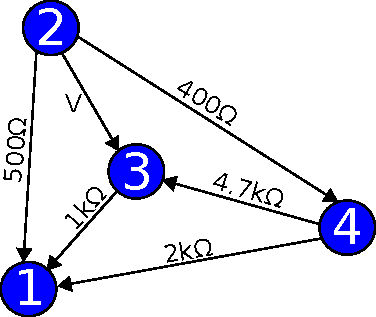
\includegraphics[scale=0.6]{Abbildungen/elektro.pdf}
		\caption{Beispiel Stromkreis (Graph).}
	\end{center}
\end{figure}
\noindent
An den elektrischen Widerst\"anden jeder Kante k\"onnen wir in Abbildung 3.2 die Korrespondenz zu Abbildung 3.1 erkennen. Die Kehrwerte der Widerst\"ande entsprechen der Kantenfunktion $r$ und $\partial=\{2, 3\}$, $g(2)=5$, $g(3)=0$ und $f\equiv 0$. Das $V$ steht f\"ur die Spannungsquelle beziehungsweise die Randbedingung.\\
\begin{center}
$
\Delta_r  = \text{grad}.T * r * \text{grad} = 
\begin{pmatrix}
1 & -1 & 0 & 0\\
1 & 0 & -1 & 0\\
1 & 0 & 0 & -1\\
0 & -1 & 1 & 0\\
0 & 0 & 1 & -1\\
0 & -1 & 0& 1\\
\end{pmatrix}^T
\begin{pmatrix}
\frac{1}{500}& 0 &0& 0& 0&0\\
0& \frac{1}{1000} & 0 & 0 &0&0\\
0 & 0 & \frac{1}{2000} & 0 &0&0\\
0 & 0 & 0 & V & 0&0\\
0 & 0 & 0 & 0 & \frac{1}{4700}&0\\
0 & 0 & 0& 0 & 0 &\frac{1}{400}\\
\end{pmatrix}
\begin{pmatrix}
1 & -1 & 0 & 0\\
1 & 0 & -1 & 0\\
1 & 0 & 0 & -1\\
0 & -1 & 1 & 0\\
0 & 0 & 1 & -1\\
0 & -1 & 0& 1\\
\end{pmatrix}=
\begin{pmatrix}
	\frac{1}{500} + \frac{1}{1000} + \frac{1}{2000}& -\frac{1}{500}  & -\frac{1}{1000} & -\frac{1}{2000}\\
	-\frac{1}{500}  & \frac{1}{500} + V + \frac{1}{400} & -V & -\frac{1}{400}\\
	-\frac{1}{1000} & -V& \frac{1}{1000} + V + \frac{1}{4700} & -\frac{1}{4700} \\
	-\frac{1}{2000} & -\frac{1}{400}&-\frac{1}{4700}  & \frac{1}{400} + \frac{1}{4700} + \frac{1}{2000}
\end{pmatrix}
$
\end{center}
Anschlie\ss{}end wendet man die Randbedingung an, daher man setzt die zweite Komponente des gesuchten Vektors $5$ und die Dritte Komponente $0$, dies entspricht dem streichen der mit $V$ markierten Ecken und bilden der passenden Inhomogenit\"at.
\begin{center}
	$
	\begin{pmatrix}[cc|c]
	\frac{1}{500} + \frac{1}{1000} + \frac{1}{2000} & -\frac{1}{2000} & \frac{5}{500}\\
	-\frac{1}{2000}& \frac{1}{400} + \frac{1}{4700} + \frac{1}{2000} & \frac{5}{400}
	\end{pmatrix}
	$
\end{center}
Dies entspricht genau der Matrixgleichung, die man mit den gebr\"auchlichen Methoden in der Physik zu diesem Problem erh\"alt.\\
\\
Die L\"osung des Poissonproblems erm\"oglicht es uns ein weiteres Analogon zu einem Theorem der klassischen Vektoranalysis zu formulieren.
\begin{corollary}[Helmoltz Zerlegung]
	Sei $G$ ein planarer Graph mit Orientierung dann gilt:
	$$\mathfrak{K}(G) = im(\text{grad}) \bigoplus im(\text{grad}_D)$$
\end{corollary}
\begin{proof}
	Eine Anwendung des de'Rham Komplexes und etwas elementare lineare Algebra liefert:
	$$\mathfrak{K}(G) = \text{kern}(\text{div}_D)\bigoplus\text{kern}(\text{div}_D)^\perp = \text{im}(\text{grad})\bigoplus\text{kern}(\text{div}_D)^\perp$$	
	Die Abbildung $\text{div}_D$ ist ein Isomorphismus zwischen $\text{kern}(\text{div}_D)^\perp$ und $\text{im}(\text{div}_D)$. Wir wissen auch bereits wegen des Theorems 3.2 dass der Laplace Operator des dualen Graphen $\Delta_D = \text{div}_D\circ\text{grad}_D$ ein Isomorphismus zwischen $\mathfrak{F}(G)$ und$\text{im}(\text{div}_D)$. In Kombination zeigt dies, dass $\text{grad}_D$ ein Isomorphismus zwischen $\mathfrak{F}(G)$ und $\text{kern}(\text{div}_D)^\perp$ ist.
\end{proof}
\chapter{Die Maxwell-Gleichungen}
Die Elektrodynamik beschreibt elektromagnetische Ph\"anomene als durch Felder vermittelte Wechselwirkung von Materie. Diese Felder gehorchen vier Gleichungen, Maxwell-Gleichungen, die im neunzehnten Jahrhundert durch den Schotten James Clerk Maxwell formuliert wurden. Diese partiellen Differentialgleichungen beschreiben wie sich elektromagnetische Felder in Abh\"angigkeit eines Materiestrom zeitlich entwickeln. Die Diskretisierung jener Differentialgleichungen  f\"uhrt im zweidimensionalen Fall zu einer Variante der Maxwell-Gleichungen f\"ur planare Graphen. 
\begin{definition}
	Sei $G$ ein planarer Graph, $r>0$, $\epsilon>0$, $e_0$ Kantenfunktionen, $j\in C^1(\mathbb{R}, \mathfrak{K})$ eine Kurve, $\mu>0$ und $b_0$ Fl\"achenfunktionen und $q_0$ eine Eckfunktion, dann nennt man eine Kurve $e\in C^1(\mathbb{R}, \mathfrak{K})$, eine Kurve $b\in C^1(\mathbb{R}, \mathfrak{F})$  und eine Kurve $e\in C^1(\mathbb{R}, \mathfrak{E})$, sodass f\"ur alle $t\in\mathbb{R}$ gilt:
	\begin{align}
		\text{div}(r * \epsilon * e(t)) = q(t)\\
		\text{div}_D(r^{-1} * e(t)) = -b^\prime(t)\\
		-r^{-1} * \text{grad}_D(b(t) / \mu) = \epsilon * e^\prime(t) + j(t)
	\end{align} 
	und die Anfangsbedingungen
\begin{align}
	e(0) = e_0\\
	b(0) = b_0\\
	q(0) = q_0
\end{align}
erf\"ullt sind, eine L\"osung der Maxwell-Gleichungen.
\end{definition}
\begin{remark}
	(4.1) nennt man das Gau\ss{}sche Gesetz und beschreibt wie das elektrische Feld $e$ mit seinen Quellen den elektrischen Ladungen zusammenh\"angt. Betrachtet man es von der Perspektive eines Flu\ss{}es ist die elektrische Ladung der Nettoflu\ss{} aus der Ecke.\\
	\\
	(4.2) nennt man das Faradaysche Gesetz und es beschreibt die zeitliche \"Anderung des magnetischen Feldes $b$ in Abh\"angigkeit des elektrischen Feldes. Die Kantenfunktion $r$ ist die L\"ange der Kante. $\epsilon$ und $\mu$ sind der elektrische und der magnetische Leitwert, respektive. Diese beiden Funktionen geben an wie gut die Kanten das Feld durchlassen.\\
	\\
	(4.3) nennt man das Amperesche Gesetz und beschreibt analog zum Faradayschen Gesetz wie die zeitliche \"Anderung des elektrischen Feldes vom magnetischen Feld, aber auch vom elektrischen Strom $j$ abh\"angig ist. Wenn wir das Ohmsche Gesetz $j(t) = \sigma e(t)$ annehmen, verh\"alt sich der elektrische Strom hier wie ein Reibungsterm. Wir werden sehen, dass dies tats\"achlich f\"ur Energieverlust ins W\"armebad verantwortlich ist.
\end{remark}
\noindent
Aus den Maxwell-Gleichungen ergeben sich die Erhaltungsgr\"o\ss{}en elektrische Ladung und Energie. Die Energie teilt sich in magnetische und elektrische Energie, die \"uber die Zeit innernander umgewandlet werden.
\begin{proposition}\textbf{Energieerhaltung}
	Sei $G$ ein planarer Graph, $r>0$, $\epsilon>0$, $e_0$ Kantenfunktionen, $\mu>0$ und $b_0$ Fl\"achenfunktionen, $q_0$ eine Eckfunktion und  $e:\mathbb{R}\rightarrow\mathfrak{K}(G)$ das elektrische Feld und $b:\mathbb{R}\rightarrow\mathfrak{F}(G)$ das magnetische Feld L\"osungen der Maxwell-Gleichungen, dann nennt man 
	\begin{equation}
	E = \frac{1}{2}(\sum_{a\in f} b(a)^2 /\mu(a) + \sum_{k\in E} \epsilon(k) * e(k)^2)
	\end{equation}
	die \textbf{Energie} und solange der elektrische Strom $j\equiv 0$ gilt, bleibt die Energie unver\"andert. 
\end{proposition}
\begin{proof}
	Sei $e$ und $b$ wie in der Voraussetzung des Satzes dann gilt f\"ur die Ableitung der magnetischen Energie:
	$$(\sum_{a\in f} b(a)^2 /\mu(a))^\prime = \sum_{a\in f} 2 * b(a) * b(a)^\prime /\mu(a) = -\sum_{a\in f} 2 * b(a) * \text{div}_D(r^{-1} * e)(a) /\mu(a)=$$
	$$-2 * \langle b /\mu, \text{div}_D(r^{-1} * e\rangle_{\mathfrak{F}}$$
	und f\"ur die Ableitung der elektrischen Energie:
	$$(\sum_{k\in E} \epsilon(k) * e(k)^2)^\prime = \sum_{k\in E} 2 * \epsilon(k) * e(k) * e(k)^\prime = $$
	$$-\sum_{k\in E} 2 * e(k) * (r^{-1} * \text{grad}_D(b /\mu) + j) (k)=-2 * \langle e, (r^{-1} * \text{grad}_D(b /\mu) + j) \rangle_{\mathfrak{K}}=$$
	$$2 * (\langle \text{div}_D(r^{-1} * e), b /\mu\rangle_{\mathfrak{F}} - \langle e, j\rangle_{\mathfrak{K}})$$
	Fassen wir zusammen:
	$$E^\prime = -\langle e, j\rangle_{\mathfrak{K}}$$
\end{proof}
\begin{proposition}\textbf{Kontinuit\"atsgesetz}
	Sei $G$ ein planarer Graph, $r>0$, $\epsilon>0$, $e_0$ Kantenfunktionen, $\mu>0$ und $b_0$ Fl\"achenfunktionen, $q_0$ eine Eckfunktion und  $e:\mathbb{R}\rightarrow\mathfrak{K}(G)$ das elektrische Feld und $b:\mathbb{R}\rightarrow\mathfrak{F}(G)$ das magnetische Feld L\"osungen der Maxwell-Gleichungen, dann gilt das Kontinuit\"atsgesetz:
	$$q^\prime = - \text{div}(r*j)$$
	Dies zeigt, dass die Gesamtladung erhalten bleibt.
\end{proposition}
\begin{proof}
	
	Dividiere (4.3) in Definition 4.1 durch $\epsilon$ und dann wende $\text{div}(r * \epsilon * .)$ auf (4.3) an:
	$$\text{div}(r * \epsilon * (-\epsilon^{-1} * r^{-1} * \text{grad}_D(b(t) / \mu))) = \text{div}(r * \epsilon * (e^\prime + j/\epsilon))$$
	$$0 = \text{div}(r * \epsilon * e)^\prime + \text{div}(r * j))$$
	$$0 = q^\prime + \text{div}(r * j)$$
	Summieren wir nun die obige Gleichung \"uber alle Ecken, dann heben sich die Beitr\"age der Kanten in $\text{div}(r*j)$ gegenseitig auf, da jede Kante einmal in dem $\text{div}$-Term der Ecke von der er wegzeigt und einmal im Term der Ecke auf die er zeigt vorkommt. Folglich gilt:
	$$\sum_{v\in V}q^\prime=0$$
\end{proof}
\noindent
Die Maxwell-Gleichungen sind ein System gew\"ohnlicher linearer Differentialgleichungen und als solches gibt es keine Probleme wegen Existenz und Eindeutigkeit f\"ur jeden Zeitpunkt. Dies l\"asst sich in jedem guten Buch \"uber gew\"ohnliche Differentialgleichungen nachlesen.
\begin{theorem}
	Die Maxwellgleichungen sind eindeutig l\"osbar, solange die Anfangsbedingung (4.1) erf\"ullt ist.
\end{theorem}
\begin{proof}
\end{proof}
\chapter{Potentialformulierung der Maxwellgleichungen}
Analog zum kontinuierlichen Fall lassen sich die Maxwellgleichungen auf planaren Graphen \"uber Potentiale ausdr\"ucken. 
\begin{definition}
Sei $G$ ein planarer Graph mit Orientierung dann nennt man eine Kurve $a\in C^1(\mathbb{R}, \mathfrak{K})$ ein Vektorpotential und eine Kurve $\phi\in C^1(\mathbb{R}, \mathfrak{E})$ ein Skalarpotential.\\
\\
Sei weiters $r>0$ eine Kantenfunktio auf $G$, dann definieren wir eine Transformation $T$,
die Potentiale $(\phi, a)\in C^1(\mathbb{R},\mathfrak{E})\times C^1(\mathbb{R},\mathfrak{K})$ in Felder $(e, b)\in C^1(\mathbb{R},\mathfrak{K})\times C^1(\mathbb{R},\mathfrak{F})$ \"uberf\"uhrt, durch
	\begin{align}
		\left(
		\begin{array}{c}
		b(t)\\
		e(t)
		\end{array}
		\right)=
		T(\left(
		\begin{array}{c}
		\phi(t)\\
		a(t)
		\end{array}
		\right))=
		\left(
		\begin{array}{c}
		\text{div}_D(r^{-1}a(t))\\
		-a^\prime(t) - r\text{grad}(\phi(t))
		\end{array}
		\right)
	\end{align}
 f\"ur alle $t\in\mathbb{R}$. 
\end{definition}
\noindent
Es ist hierbei zu bedenken, dass $\text{div}_D$ nicht surjektiv ist, sondern nur Fl\"achen-funktionen darstellen kann, die orthogonal zu den konstanten Funktionen sind. Dies scheint auf den ersten Blick eine Einschr\"ankung zu sein, aber eine kurze Betrachtung der Maxwellgleichungen zeigt uns, dass der konstante Anteil des Magnetfeldes keine Auswirkung auf das elektrische Feld hat, solange $\mu$ konstant ist. Viel wichtiger noch findet die einzige \"Anderung des Magnetfeldes, die unter G\"ultigkeit der Maxwellgleichungen passieren darf im orthogonalen Komplement der konstanten Fl\"achenfunktionen statt.\\
Wir fordern nun zus\"atzlich zu den Maxwellgleichungen, dass das Magnetfeld $b$
f\"ur jeden Zeitpunkt $t\in\mathbb{R}$ orthogonal zu den konstanten Fl\"achenfunktionen ist: 
$$b(t)\in \mathbb{R}^\perp$$
Wenn wir planare Graphen als Polyeder auffassen, ist dies einfach das im dreidimensionalen g\"ultige Gau\ss{}sche Gesetz f\"ur Magnetfelder.\\
\\
Die Wahl der Potential Definition kam nicht von ungef\"ahr, sondern aus der Theorie im Kontinuum. 
Die Definition des Magnetfeldes in (5.1) abgeleitet ergibt durch Einsetzen der Definition des elektrischen Feldes sofort das Faradaysche Gesetz. 
Nachdem das Gaußsche Gesetz als Definition der elektrischen Ladung gesehen werden kann, reduzieren sich die Maxwellgleichungen in Potentialformulierung auf das Amperesche Gesetz: 
\begin{equation}
r^{-1}\text{grad}_D(\text{div}_D(r^{-1}a(t)) / \mu) = \epsilon * (a^{\prime\prime} + r\text{grad}(\phi^\prime)) - j(t)
\end{equation}
Der Vorteil der Potentialdarstellung liegt zum Einen in der Vereinfachung des Gleichungssystems und zum Anderen in der gr\"o\ss{}eren Flexibilit\"at.\\
\\
Es ist leicht zu sehen, dass die Operation aus Definition 5.1, die Potentiale in Felder um wandelt nicht injektiv ist.\\
\\
Die Charakterisierung des Kerns dieser linearen Operation f\"uhrt uns nun zu den so genannten Eichtransformationen.
\begin{definition}
	Seien $\phi$ und $a$ Potentiale wie in Definition 5.1, und $\xi\in C^1(\mathbb{R}, \mathfrak{E})$, dann nennt man die Transformation $T$ definiert durch
\begin{equation}
\gamma_\xi(\left(
\begin{array}{c}\phi\\
a
\end{array}\right))=
\left(
\begin{array}{c}\phi - \xi^\prime\\
a + r\text{grad}(\xi) 
\end{array}\right)
\end{equation}
	die zu $\xi$ geh\"orende \textbf{Eichtransformation}.
\end{definition}
\noindent
Die Potentiale werden immer genau bis auf eine Eichtransformation eindeutig durch die Felder bestimmt.
\begin{proposition}
	Sei $T$ die lineare Operation aus Definition 5.1, die Potentiale $(\phi, a)\in C^1(\mathbb{R},\mathfrak{E})\times C^1(\mathbb{R},\mathfrak{K})$ in Felder $(e, b)\in C^1(\mathbb{R},\mathfrak{K})\times C^1(\mathbb{R},\mathfrak{F})$ \"uberf\"uhrt, dann gilt:
	\begin{equation}
	\text{kern}(T)=\{\left(
	\begin{array}{c}-\xi^\prime\\
	r\text{grad}(\xi)
	\end{array}\right)| \xi\in C^1(\mathbb{R},\mathfrak{E})\}
	\end{equation}
\end{proposition}
\begin{proof}
Wir starten mit der Inklusion $(\supset)$\\
Sei $(\phi, a)\in \text{kern}(T)$, dann gilt f\"ur alle $t\in\mathbb{R}$
\begin{equation*}
	0 = \text{div}_D(r^{-1}a(t))
\end{equation*} 
Wir wissen wegen dem de'Rham Komplex Theorem, und weil $r>0$ ist, dass es eine  $\chi:\text{im}(\text{grad})\mapsto \mathbb{R}^\perp$ gibt, sodass gilt:
\begin{equation*}
	x = \text{grad}(\chi(x)) \text{ f\"ur  alle }x\in\mathfrak{K}(G)
\end{equation*}
Daher k\"onnen wir f\"ur alle $t\in\mathbb{R}$ definieren 
\begin{equation*}
\xi(t) = \chi(r^{-1}a(t))
\end{equation*} sodass gilt
\begin{equation*}
	a=r\text{grad}(\xi)
\end{equation*} und $\xi\in C^1(\mathbb{R},\mathfrak{E})$.\\
Wir setzen den so gewonnenen Ausdruck f\"ur $a$ nun ein in
\begin{equation*}
	0=-a^\prime(t) - r\text{grad}(\phi(t))
\end{equation*} 
und erhalten f\"ur alle $t\in\mathbb{R}$
\begin{equation*}
0=\text{grad}(\xi^\prime(t)+\phi(t))
\end{equation*} 
Somit gilt die Gleichheit modulo einer Konstante $c$
\begin{equation*}
\phi(t)=-\xi^\prime(t) +c
\end{equation*}
Die Konstante $c$ kann man weil sie im Kern des Gradienten liegt in $\xi$ einziehen.
\begin{equation*}
	\xi(t) = \chi(r^{-1}a(t)) -c*t
\end{equation*}
\noindent
Die andere Inklusion $(\subset)$ wird gezeigt indem man den Ausdruck in der Mengendefinition (5.4) in $T$ eingesetzt wird.
\end{proof}
\noindent
Hiermit wurden die wichtigsten Aspekte der Potentialdarstellung vorgestellt. Dies ist eine Grundvoraussetzung f\"ur die Quantisierung der Maxwellgleichungen.
\chapter{Kanonische Quantisierung des elektromagnetischen Feldes}
Anfang des zwanzigsten Jahrhunderts wurde zur Erkl\"arung einer Reihe von Ph\"anomenen, die innerhalb der damals etablierten/klassischen physikalischen Theorien nicht erkl\"arbar waren, die Quantentheorie entwickelt.
Die Objekte der klassischen Theorien sind Kurven, Kr\"afte und Felder und in der Quantenmechanik sind es Zustandsvektoren, Operatoren und Distributionen. Die messbaren Gr\"o\ss{}en bleiben dieselben, allerdings werden die mathematischen Objekte, die ihr Verhalten beschreiben etwas komplizierter.\\
\\
Wir wollen nun den klassischen Weg der Quantisierung einer physikalischen Theorie am Beispiel der Maxwellgleichungen auf planaren Graphen erkunden.\\
\\
Der Ausgangspunkt dieser so genannten kanonischen Quantisierung ist die Lagrangefunktion der Theorie.
\begin{theorem}
Sei $G$ ein planarer Graph, $r>0$, $\epsilon>0$,  Kantenfunktionen, $j\in C^1(\mathbb{R}, \mathfrak{K})$, $\mu>0$ eine Fl\"achenfunktion dann sind $a$ und $\phi$ L\"osungen der Maxwellgleichung in Potentialform (5.2), genau dann wenn alle Richtungsableitungen des Wirkungsfunktionals verschwinden auf dem Raum der $f_1\in C^1(\mathbb{R}, \mathfrak{E})$ und $f_2\in C^1(\mathbb{R}, \mathfrak{K})$ f\"ur die gilt, dass $f_1$ und $\phi$ sowie $f_2$ und $a$ zu den Zeitpunkten $r$ und $s$ \"ubereinstimmen
\begin{equation}
	S(f_1, f_2) = \int_{r}^{s}W(f_1, f_2, f_1^\prime, f_2^\prime)dt
\end{equation}
\noindent
Die Funktion unter dem Integral nennt man die \textbf{Lagrangefunktion} der Maxwellgleichung.
Sie ist dabei gegeben durch:
\begin{align*}
	L(q_1, q_2, v_1, v_2) =&\frac{1}{2}(\langle \epsilon(v_2 + r\text{grad}(q_1)), v_2 + r\text{grad}(q_1)\rangle_\mathfrak{K} -\\& \langle\text{div}_D(r^{-1}q_2), \text{div}_D(r^{-1}q_2)/\mu\rangle_\mathfrak{K}) + \langle q_2, j\rangle_\mathfrak{K}
\end{align*}
\end{theorem}
\begin{proof}
Siehe beliebiges Fachbuch zur theoretischen Physik.
\end{proof}
\noindent
Im n\"achsten Schritt wollen wir diese Lagrangefunktion \"uber eine Legendre Transformation in die zugeh\"orende \textbf{Hamiltonfunktion} umgewandelt.
\begin{definition}
	Sei $f:X\mapsto\mathbb{R}$ eine konvexe Funktion auf einem Skalarproduktraum $X$, dann ist die \textbf{Legendretransformation} $f^*$ definiert durch:
	\begin{equation}
		f^*(y) = \sup_{x\in X}(\langle x, y\rangle-f(x))
	\end{equation}
\end{definition}
\noindent
Zuvor sollte aber noch eine kleine Modifikation an der Lagrangefunktion vorgenommen werden um eine sch\"one geschlossene Darstellung der Hamiltonfunktion zu erhalten.
\begin{proposition}
	Sei $f:X\mapsto\mathbb{R}$ eine strikt konvexe stetig differenzierbare Funktion auf einem Skalarproduktraum $X$, sodass die Abbildung $x\mapsto Df(x)$ invertierbar ist, dann ist die Legendretransformation gegeben durch:
	\begin{equation}
		f^*(y) = \langle (Df)^{-1}(y), y\rangle-f((Df)^{-1}(y))
	\end{equation}
\end{proposition}
\begin{proof}
Die Funktion $g_y(x)=\langle x, y\rangle-f(x)$ ist streng konkav und hat daher ein eindeutiges Maximum $x_0\in X$.
\begin{equation*}
	Dg_y(x_0) = y - Df(x_0)=0\Rightarrow x_0 = (Df)^{-1}(y)
\end{equation*}
Eingesetzt in $g_y$ erhalten wir dann
\begin{equation*}
	f^*(y)=g_y(x_0) = \langle (Df)^{-1}(y), y\rangle-f((Df)^{-1}(y))
\end{equation*}
\end{proof}
\noindent
Um diese Darstellung ausnutzen zu k\"onnen m\"ussen wir das Skalarpotential $\phi$ aus der Lagrangefunktion entfernen.\\
Dies ist m\"oglich, da es zu jeder Paarung eines Skalarpotentials und eines Vektorpotentials eine Eichtransformation gibt, die diese in ein Paar umwandelt, dessen Skalarpotential gleich Null ist.\\
\\
Die resultierende Lagrangefunktion ist gegeben durch 
\begin{equation}
	L(q, v) =\frac{1}{2}(\langle \epsilon v, v\rangle_\mathfrak{K} - \langle\text{div}_D(r^{-1}q), \text{div}_D(r^{-1}q)/\mu\rangle_\mathfrak{K}) + \langle q, j\rangle_\mathfrak{K}
\end{equation}
\noindent
Das \"ubrige Vektorpotential (hier q) ist immer noch nicht eindeutig bestimmt, und die Eichtransformationen die diese Form der Eichung erhalten sind genau jene, die laut Definition (5.2) zu einem konstanten $\xi$ korrespondieren.\\
\\
Die Hamiltonfunktion erhalten wir durch eine Anwendung der Legendretransformation auf die Lagrangefunktion (6.4) bez\"uglich der Variablen $v$.
\begin{equation}
	H(\pi, q) = \frac{1}{2}\langle \frac{\pi}{\epsilon}, \pi\rangle_{\mathfrak{K}} + \frac{1}{2}\langle \text{div}_D(r^{-1}q), \text{div}_D(r^{-1}q)/\mu\rangle_{\mathfrak{K}} - \langle q, j\rangle_{\mathfrak{K}}
\end{equation}
Wenn wir mit (4.7) der Energieerhaltung, Satz (4.1), vergleichen, erkennen wir, dass, die ersten beiden Terme genau die dort proklamierte Gesamtenergie sind und der \"ubrige Term genauso so beschaffen scheint um die zeitliche Ableitung nach Satz 4.1 zu kompensieren. Solange $j$ zeitunabh\"anging ist, und somit auch $H$ nicht explizit von der Zeit abh\"angt, ist dies auch der Fall.\\
\\
Mit Hilfe der Euler-Lagrange-Gleichung k\"onnen wir nun die \textbf{Hamiltonschen Bewegungsgleichungen} herleiten.
\begin{proposition}
Sei $G$ ein planarer Graph, $r>0$, $\epsilon>0$,  Kantenfunktionen, $j\in C^1(\mathbb{R}, \mathfrak{K})$, $\mu>0$ eine Fl\"achenfunktion dann sind $a$ und $\phi$ L\"osungen der Maxwellgleichung in Potentialform (5.2), genau dann wenn die Hamiltonschen Bewegunggleichungen erf\"ullt sind:
\begin{align}
	q^\prime = \frac{\partial H}{\partial \pi}\\
	\pi^\prime = - \frac{\partial H}{\partial q}
\end{align}
\end{proposition}
\begin{proof}
	Siehe beliebiges Fachbuch zur theoretischen Physik.
\end{proof}
\noindent
An diesem Punkt entfernen wir uns von der klassischen Theorie und folgen Heisenberg in die Quantenmechanik. Die Kurven $\pi$ und $q$ aus $C^1(\mathbb{R}, \mathfrak{K})$ sind von nun an Kurven $\hat{\pi}$ und $\hat{q}$ in einem Raum von Operatoren auf einem Hilbertraum.
\begin{definition}
	Sei $G$ ein planarer Graph und $r>0$ eine Kantenfunktion, dann ist der Hilbertraum unserer Theorie gegeben durch
	\begin{equation}
		\mathfrak{H} = L^2(\mathfrak{K}(G),\mathbb{C};\lambda)
	\end{equation}
	Der Raum der komplexen Funktionen auf $\mathfrak{K}(G)$ deren Quadrate ein endliches Integral bez\"uglich dem Ma\ss{} $\lambda$\footnote{$\lambda$ wird zu einem sp\"ateren Zeitpunkt festgelegt.} hat.\\
	\\
	Das Skalarprodukt auf $\mathfrak{H}$ ist dabei definiert durch:
	\begin{equation}
		\langle \phi, \xi\rangle_{\mathfrak{H}} = \int_\mathfrak{K} \overline{\phi}(q)\xi(x)d\lambda(x)
	\end{equation}
\end{definition}
\noindent
\paragraph{Interpretation}
\begin{itemize}
\item Jedes Element $\psi\in\mathfrak{H}$ stellt einen m\"oglichen Zustand des quantisierten elektromagnetischen Feldes dar. 
\item Jeder Messgr\"o\ss{}e $\Omega$ des klassischen elektromagnetischen Feldes entspricht ein korrespondierender Operator $\hat{\Omega}$ auf $\mathfrak{H}$. 
\item Der Ausgang einer Messung der Gr\"o\ss{}e $\Omega$ ist zuf\"allig und der Mittelwert der Messungen ist gleich $\frac{\langle \psi, \hat{\Omega}\psi\rangle_{\mathfrak{H}}}{\langle \psi, \psi\rangle_{\mathfrak{H}}}$.
\end{itemize}
\noindent
Widmen wir uns nun der Konstruktion der korrespondierenden Operatoren. Nach Heisenberg wird f\"ur jedes Kantenpaar $e,e'\in E$ die kanonische Vertauschungsrelation:
\begin{equation}
	[\hat{q}(e), \hat{\pi}(e')] = i\delta_{e, e'}
\end{equation}
gefordert.\\
\\
Eine m\"ogliche Darstellung dieser Operatoren $\hat{q}(k)$ und $\hat{\pi}(k)$, die (6.10) erf\"ullt ist gegeben durch:
\begin{align}
	\hat{\pi}(k):(q\mapsto\psi(q)) \mapsto (q\mapsto -i\frac{\partial\psi}{\partial q_k}(q))\text{  f\"ur }k\in E\\
	\hat{q}(k):(q\mapsto\psi(q)) \mapsto (q\mapsto q_k\psi(q))\text{  f\"ur }k\in E
\end{align}
\noindent
Hierbei ist $q_k$ der Wert der Kantenfunktion $q$ an der Stelle $k\in E$ und $\frac{\partial}{\partial q_k}$ ist die Ableitung nach demselben Wert.
\\
\\
Eine kurze Betrachtung der Hamiltonfunktion (6.4) zeigt die \"Aquivalenz dieses Problems zu der Bewegung von $|E|$ Punktma\ss{}en mit Massen $\epsilon(k)$ f\"ur jedes $k\in E$ in einem Potential. 
\begin{definition}
	Sei $G$ ein planarer Graph, $r>0$, $\epsilon>0$, $e_0$ Kantenfunktionen, $\hat{j}$ eine Kurve selbstadjungierter Operatoren auf $\mathfrak{H}(G)$, $\mu>0$ und $b_0$ Fl\"achenfunktionen, dann ist der der Hamiltonoperator des elektromagnetischen Feldes gegeben durch:
	\begin{equation}
	\hat{H}=-\sum_{k\in E}\frac{1}{2\epsilon(k)}\frac{\partial^2}{\partial q_k^2} + \frac{1}{2}\langle \text{div}_D(r^{-1}q), \text{div}_D(r^{-1}q)/\mu\rangle_{\mathfrak{K}} - \langle q, \hat{j}\rangle_{\mathfrak{K}}
	\end{equation}
	Sei $\psi_0\in\mathfrak{H}$ und $\psi\in C^1(\mathbb{R},\mathfrak{H})$, sodass:
\begin{equation}
\hat{H}\psi(t) = i\psi^\prime(t)
\end{equation}
f\"ur alle $t\in\mathbb{R}$ gilt und die Anfangsbedingung $\psi(0)=\psi_0$ erf\"ullt ist, dann nennt man $\psi$ eine L\"osung der
\textbf{Schr\"odingergleichung}.
\end{definition}
\noindent
Es wird Zeit einen Gang runter zu schalten und zu analysieren was wir gewonnen haben. Hierzu geh\"ort es im ersten Schritt zu zeigen, dass die durch die Schr\"odingergleichung vermittelte Dynamik im Mittel mit jener der Maxwellgleichungen \"ubereinstimmt. 
\begin{theorem}[Ehrenfest Theorem]
	Sei $G$ ein planarer Graph, $\epsilon>0$ und $r>0$ Kantenfunktionen, $\mu>0$ eine Fl\"achenfunktion und $\psi: \mathbb{R}\mapsto \mathfrak{H}$ eine L\"osung der Schr\"odingergleichung (6.14) auf $G$, dann gilt:
	\begin{align}
		&\epsilon\langle \psi, \hat{e}\psi\rangle_{\mathfrak{H}}^\prime =  -r^{-1} \text{grad}_D(\langle\psi,\hat{b}\psi\rangle_{\mathfrak{H}}/\mu) -  \langle \psi, \hat{j} \psi\rangle_{\mathfrak{H}}\\
		&\langle \psi, (\hat{b}\psi)\rangle_{\mathfrak{H}}^\prime = -\text{div}_D(r^{-1}\langle\psi, \hat{e}\psi\rangle_{\mathfrak{H}})
	\end{align}
	wobei der elektrische und magnetische Feldoperator gegeben sind durch:
	\begin{align}
		&\hat{e} = \frac{-\hat{\pi}}{\epsilon}\\
		&\hat{b} = \text{div}_D(r^{-1}\hat{q})
	\end{align}
\end{theorem}
\begin{proof}
Wir starten mit der linken Seite von (6.15), wenden die Produktregel der Differentiation an und formen um:
\begin{align*}
	&\epsilon\langle \psi, \hat{e}\psi\rangle_{\mathfrak{H}}^\prime = -\langle \psi, \hat{\pi}\psi\rangle_{\mathfrak{H}}^\prime=\\
	&-(\langle \psi^\prime, \hat{\pi}\psi\rangle_{\mathfrak{H}}+\langle \psi, \hat{\pi}\psi^\prime\rangle_{\mathfrak{H}})=\\
	&\langle i\hat{H}\psi, \hat{\pi}\psi\rangle_{\mathfrak{H}}+\langle \psi, \hat{\pi}i\hat{H}\psi\rangle_{\mathfrak{H}})=\\
	&i(\langle \psi, \hat{\pi}\hat{H}\psi\rangle_{\mathfrak{H}} - \langle \hat{H}\psi, \hat{\pi}\psi\rangle_{\mathfrak{H}})=\\
	&i(\langle \psi, \hat{\pi}\hat{H}\psi\rangle_{\mathfrak{H}} - \langle \psi, \hat{H}\hat{\pi}\psi\rangle_{\mathfrak{H}})=\\
	&-r^{-1} \text{grad}_D(\langle\psi,\text{div}_D(r^{-1}\hat{q})\psi\rangle_{\mathfrak{H}}/\mu) -  \langle \psi, \hat{j} \psi\rangle_{\mathfrak{H}}\\
	&-r^{-1} \text{grad}_D(\langle\psi,\hat{b}\psi\rangle_{\mathfrak{H}}/\mu) -  \langle \psi, \hat{j} \psi\rangle_{\mathfrak{H}}
\end{align*}
Nun zeigen wir (6.16) indem wir ausgehend von (6.18) die Formel
	\begin{align}
\langle \psi, \hat{b}\psi\rangle_{\mathfrak{H}}^\prime = \text{div}_D(r^{-1}\langle \psi, \hat{q}\psi\rangle_{\mathfrak{H}}^\prime)
\end{align}
ableiten. Anschließend wenden wir wieder die Produktregel auf den Ausdruck $\langle \psi, \hat{q}\psi\rangle_{\mathfrak{H}}^\prime$ an und formen um
	\begin{align*}
	&\langle \psi, \hat{q}\psi\rangle_{\mathfrak{H}}^\prime= (\langle \psi^\prime, \hat{q}\psi\rangle_{\mathfrak{H}}+\langle \psi, \hat{q}\psi^\prime\rangle_{\mathfrak{H}})=\\
	&i(\langle \psi, \hat{H}\hat{q}\psi\rangle_{\mathfrak{H}} - \langle \psi, \hat{q}\hat{H}\psi\rangle_{\mathfrak{H}})=\\
	&i\langle \psi, [\hat{H},\hat{q}]\psi\rangle_{\mathfrak{H}}=i\langle \psi, [\frac{1}{2\epsilon}\hat{\pi}^2,\hat{q}]\psi\rangle_{\mathfrak{H}}\\
	&\langle \psi, \frac{\hat{\pi}}{\epsilon}\psi\rangle_{\mathfrak{H}}=-\langle \psi, \hat{e}\psi\rangle_{\mathfrak{H}}
\end{align*}		
Am Ende haben wir hier die kanonischen Vertauschungsrelationen und die Rechenregeln des Kommutators verwendet.
Wir setzen den erhaltenen Ausdruck nun in (6.19) ein und erhalten das gesuchte Resultat.
\end{proof}
\noindent
Wir sehen also, dass die Schr\"odingergleichung (6.14) tats\"achlich eine Quantisierung der Maxwellgleichungen (4.1) darstellt.
\iffalse
Als n\"achstes soll die Eichinvarianz der freien Schr\"odingergleichung also mit $\hat{j}=0$ untersucht werden.
\begin{theorem}
	Sei $G$ ein planarer Graph, $\epsilon>0$ und $r>0$ Kantenfunktionen, $\mu>0$ eine Fl\"achenfunktion und $\psi: \mathbb{R}\mapsto \mathfrak{H}$ eine L\"osung der Schr\"odingergleichung (6.14) auf $G$, dann kommutiert das folgende Diagramm f\"ur jedes $\xi\in\mathfrak{E}$ und $x\in\mathfrak{K}$:\\
	\begin{tikzcd}
		\psi(x,t) \arrow{d}{+\Delta t}\arrow{r}{+r\text{grad}(\xi)} & \psi(x+r\text{grad}(\xi),t) \arrow{d}{+\Delta t}\\
		\psi(x,t+\Delta t) \arrow{r}{+r\text{grad}(\xi)}& \psi(x+r\text{grad}(\xi),t+\Delta t) \\
	\end{tikzcd}
\end{theorem}
\begin{proof}
\end{proof}
\noindent
TODO\\
\fi
Bislang haben wir noch keine Bestätigung, dass die Schr\"odingergleichung (6.14) l\"osbar ist oder der Hamiltonoperator $\hat{H}$ selbstadjungiert im Sinne der Theorie unbeschr\"ankter linearer Operatoren ist. Dies wollen wir f\"ur den Fall $\epsilon\equiv 1$ und $\mu\equiv 1$ nachholen.
\begin{theorem}
	Sei $G$ ein planarer Graph, $\epsilon\equiv 1$ und $r>0$ Kantenfunktionen, $\mu\equiv 1$ eine Fl\"achenfunktion, dann existiert eine unit\"are Abbildung $\hat{U}$ auf $\mathfrak{H}$ und $(\omega_j)_{j=1}^{|f|-1}>0$ sodass f\"ur den Hamiltonoperator $\hat{H}$ (6.13) mit $\hat{j}\equiv 0 $ gilt:
	\begin{equation}
	\hat{U}^\dagger\hat{H}\hat{U}  = \sum_{j=1}^{|E|}h_j
	\end{equation}
Wobei die $h_j$ gegeben sind durch:
\[h_j= \begin{cases} 
-\frac{1}{2}\frac{\partial^2}{\partial x_j^2} & j\leq |V| - 1 \\
-\frac{1}{2}\frac{\partial^2}{\partial x_j^2} + \frac{1}{2}\omega_j x_j^2 & \text{sonst.} 
\end{cases}
\]
\end{theorem}
\begin{proof}
	Der Hamiltonoperator l\"asst sich folgenderma\ss{}en zerlegen:
	\begin{equation*}
		\hat{H} = \hat{T} + \hat{V}
	\end{equation*}
	wobei
	\begin{align*}
		&\hat{T} = -\frac{1}{2}\sum_{k\in E}\frac{\partial^2}{\partial q_k^2}\\
	    &\hat{V} = \frac{1}{2}\langle \text{div}_D(r^{-1}q), \text{div}_D(r^{-1}q)\rangle_{\mathfrak{K}}
	\end{align*}
	Wir formen nun $\hat{V}$ um
	\begin{align*}
		&\frac{1}{2}\langle \text{div}_D(r^{-1}q), \text{div}_D(r^{-1}q)\rangle_{\mathfrak{K}}=\\
		&\frac{1}{2}\langle q, (-r^{-1}\text{grad}_D\text{div}_D)(r^{-1}q)\rangle_{\mathfrak{K}}=
	\end{align*}
	und f\"uhren einen linearen Operator $Q=-r^{-1}\text{grad}_D\text{div}_Dr^{-1}$ ein
	\begin{align}
		&\frac{1}{2}\langle q, Q(q)\rangle_{\mathfrak{K}}
	\end{align}
	$Q$ ist positiv semidefinit und symmetrisch. Die Dimension des Kerns von $Q$ ist nach der Helmoltz Zerlegung (3.3) gleich $|V| - 1$. Das orthogonale Komplement desselben Kerns ist entsprechend $|f| - 1$ dimensional.\footnote{Der eulersche Polyedersatz ist eine Folgerung der Helmoltz Zerlegung.}
	Nach dem Spektralsatz linearer Operatoren auf endlich dimensionalen komplexen Vektorr\"aumen l\"asst sich $Q$ schreiben als:
	\begin{equation*}
		Q = U^\dagger R U
	\end{equation*}
	Die Diagonalmatrix $R$ is nicht-negativ und hat genau $|f| - 1$ positive Eintr\"age.\\
	Ein wenig umformen von (6.20) liefert dann
	\begin{align*}
		&\frac{1}{2}\langle q, Q(q)\rangle_{\mathfrak{K}}=\\
		&\frac{1}{2}\langle q, U^\dagger R U(q)\rangle_{\mathfrak{K}}=\\
		&\frac{1}{2}\langle U(q), R U(q)\rangle_{\mathfrak{K}}
	\end{align*}
	Wir k\"onnen $U$ und $r$ so w\"ahlen, dass die ersten $|V|-1$ Eintr\"age Null sind und definieren 
	\begin{equation*}
		\omega_j = R_{|V|-1 + j} \text{ f\"ur }1\leq j \leq |f| - 1
	\end{equation*}
	Wir konstruieren nun den unit\"aren Operator $\hat{U}$. Sei $\phi\in\mathfrak{H}$ und $q\in\mathfrak{K}$
	\begin{equation*}
		\hat{U}(\phi)(q)=\phi(U(q))
	\end{equation*}
	Der Operator $\hat{U}$ ist offensichtlich invertierbar und weil $U$ unit\"ar auf $\mathfrak{K}$ ist nach dem Transformationssatz f\"ur Integrale auch unit\"ar.\\
	\\
		Der Operator $\hat{T}$ ist der Laplaceoperator und somit invariant unter orthogonaler Transformation.\\
	\\
	F\"ur den Operator $\hat{V}$ kann die gesuchte Transformationseigenschaft (6.19) durch einige wenige Umformungen gezeigt werden.
	\begin{align*}
		&(\hat{U}^\dagger\hat{V}\hat{U})(\phi)(q)= \\
		&\hat{U}^\dagger(\frac{1}{2}\langle U(q), R U(q)\rangle_{\mathfrak{K}}\phi)(U(q))=\\
		&\frac{1}{2}\langle U^\dagger U(q), R U^\dagger U(q)\rangle_{\mathfrak{K}}\phi(U^\dagger U(q))\\
		&\frac{1}{2}\langle q, R q\rangle_{\mathfrak{K}}\phi(q)
	\end{align*}

\end{proof}
\noindent
Wir haben nun gezeigt, dass sich der freie Hamiltonoperator (6.13), daher mit $\hat{j}\equiv 0$, zerlegen l\"asst in eine endliche Summe von selbst-adjungierten Operatoren mit bekannten Spektra.\\
\\
Daraus folgt direkt die Existenz und Eindeutigkeit von L\"osungen mit beliebigen Anfangsbedingungen.
\begin{theorem}
	Sei $G$ ein planarer Graph, $\epsilon\equiv 1$ und $r>0$ Kantenfunktionen, $\mu\equiv 1$ eine Fl\"achenfunktion, dann gibt es eine eindeutige L\"osung der Schr\"odingergleichung.
\end{theorem}
\chapter{Zweite Quantisierung des elektromagnetischen Feldes}
Das elektromagnetische Feld tauscht Energie mit Materie in Quanten also festen Portionen aus. Diese Portionen nennt man Photonen und die Energie $E$ eines Photons ist proportional zu seiner Frequenz $\nu$. Diese Eigenschaft der Quantentheorie des elektromagnetischen Feldes spiegelt sich noch nicht in unserer Beschreibung wieder.\\
\\
Unsere bisheriges Modell beschreibt ein einzelnes Photon. Wir erweitern es nun zu einem Multi-Photonen-Modell.
\begin{definition}
	Sei $\mathfrak{H}$ der Ein-Photonen-Hilbertraum aus Definition (6.3), dann definieren wir den symmetrischen Tensorprodukt-Raum rekursiv als
	\begin{align}
		&\mathfrak{H}^0 = \mathbb{C}\\
		&\mathfrak{H}^n = S(\mathfrak{H}^{n-1}\otimes\mathfrak{H})
	\end{align}
	wobei f\"ur jedes $m\geq 1$ und jedes $\phi\in\mathfrak{H}^m$ $S$ definiert ist durch \begin{equation}
		S(\phi)(x_1,\dots,x_m)=
		\frac{1}{N!}\sum_{\sigma\in\text{Aut}([m])}\phi(x_{\sigma(1)},\dots,x_{\sigma(m)})
	\end{equation}
	Der \textbf{Fockraum} ist dann definiert als die direkte Summe der symmetrischen Tensorprodukte
	\begin{equation}
		F(\mathfrak{H})=\oplus_{j\geq 0}\mathfrak{H}^j
	\end{equation}
	Der Fockraum ist der Raum der Zust\"ande mit beliebiger Teilchenanzahl.
\end{definition}
\noindent
Der Raum der symmetrischen Tensorprodukte wird gew\"ahlt, da Photonen ununterscheidbar sind und daher kein Zustand existieren kann indem ein Photon ausgezeichnet ist.\\
\\
Einen Zustand mit Null Teilchen nennt man Vakuumzustand.\\
\\
\chapter{Die Klein-Gordongleichung und ihr Eichfeld}
\chapter{Quantisierung der Klein-Gordongleichung}
\chapter{Quantenelektrodynamik des planaren Graphen}
\chapter*{Abschluss}
Es hat mich sehr gefreut diese Arbeit zu schreiben. Ich wei\ss{} nicht wirklich ob sie jemals jemandem n\"utzlich sein wird, aber falls ja w\"urde mich das sehr freuen. Im dreidimensionalen ist alles eine Spur komplizierter, aber in einigen Punkten auch wieder nicht. Elektromagnetismus passt halt recht gut zu drei Raumdimensionen. Besonders wichtig am Schluss war es mir zu zeigen, warum Widerstandsnetzwerke so nett l\"osbar sind, und aber auch das man von der Intuition von elektrischen Netzwerken die dicht den Raum erf\"ullen alle elektromagnetischen Ph\"anomene beschreiben kann. Eine Diskretisierung (Finite Differenzen) der Maxwellgleichungen der Ebene entspricht genau den Maxwellgleichungen die im letzten Kapitel entwickelt wurden. \\
\\
Es war sehr sch\"on, es hat mich sehr gefreut!
\end{document}

